\documentclass{report}
% pre\'ambuloasdf

\usepackage{lmodern}
\usepackage[T1]{fontenc}
\usepackage[10pt]{moresize}
\usepackage{amsmath} 
%\usepackage{fontspec}
%\setmainfont{Times New Roman}
\usepackage[spanish,activeacute]{babel}
\usepackage{mathtools}
\usepackage{graphicx}
%\usepackage{anysize} 
\usepackage[%
    left=1.2in,%
    right=1.2in,%
    top=1.7in,%
    bottom=1.5in,%
    paperheight=11in,%
    paperwidth=8.5in%
]{geometry}

\title{TFG}
\author{Jorge Vela Pe?a}

\begin{document}
% cuerpo del documento


\large
%\marginsize{3cm}{2cm}{2cm}{2cm} 

%\rmfamily

\chapter{Infraestructura utilizada.}
En esta parte voy a hablar sobre los diferentes elementos y aplicaciones para el desarrollo de este proyecto.

\hspace{1 cm} En primer lugar hay que hablar del \textbf{Parrot AR.Drone 2.0}, dron utilizado para realizar las pruebas y poder comprobar de esta manera que el desarrollo del programa era el correcto. 

\hspace{1 cm} La \textsl{bater\'ia} de este era de 1500mah, lo que en algunas ocasiones nos ha llevado a problemas, pues el tiempo de vuelo con esto es unos 12 minutos aproximadamente. Esto conllevaba que algunas pruebas en ocasiones eran muy dif\'iciles de realizar, ya que si no salia el resultado esperado en los primeros intentos muchas veces hab\'ia que parar la prueba durante bastante rato para continuar. Si las pruebas no eran de vuelo sino que era de imagen con este tiempo era suficiente, ya que el dron no gastaba tanta energ\'ia al relizar solo la retransmisi\'on de los datos que obten\'ia la c\'amara. Un detalle curioso en este punto es el cambio de funcionamiento que se notaba una vez la bater\'ia estaba por debajo del 30/100, pues el despegue se hacia con menos fuerza y de forma m\'as inestable, adem\'as las instrucciones de movimiento que se le mandaban las ejecutaba con menos fuerza y por lo tanto de forma m\'as lenta. La \'unica soluci\'on posible para remediar este problema fue trabajar a la vez con 3 baterias, pero he de decir que en momentos que las pruebas eran muy continuas durante mucho tiempo, llegaba un momento que hab\'ia que parar porque el tiempo de carga no era suficientemente rapido comparado con el de las 3 descargas. 

\hspace{1 cm} El \textsl{alcance} que tiene \'este con la estaci\'on tierra es de 50 metros, suficiente para las pruebas que han sido realizadas en este proyecto. 

\hspace{1 cm} Este dron tiene una \textsl{placa base} ARM Cortex A8 de 1Ghz y un DSP de v\'ideo de 8Ghz. Tambi\'en posee una memoria RAM DDR2 de 1GB y 200Mhz. Este chip es el encargado de levantar una red WiFi, a la cual nos podemos conectar mediante el smartphone (hay una aplicacion espec\'ifica para ello), o como en este caso, mediante el ordenador, y de esta forma poder controlarlo. Esta placa base funciona con Linux. 

\hspace{1 cm} Adem\'as, dicho dron cuenta con dos \textsl{c\'amaras}, una horizontal y otra vertical, lo que nos permite ver diversos planos en todo momento. Estas c\'amaras est\'an conectadas a la placa base, lo que permite en todo momento la transmisi\'on de im\'agenes en directo, gracias a las cuales podremos trabajar, sera la informaci\'on gracias a la cual podremos darle instrucciones al dron. Cabe destacar la diferencia de calidad que hay entre las c\'amaras, algo que se notaba al realizar pruebas con una c\'amara, y cuando todo era correcto y querias cambiar de c\'amara para realizar otra prueba se pod\'ia observar como los colores perdian nitidez y se despreciaban algunos detalles, lo que te llevaba a cambiar cosas de los algoritmos que en un principio no se esperaban. 

\hspace{1 cm} Ya para terminar, la \textsl{velocidad} de este drone puede llegar a alcanzar los 18km/h, algo que en este proyecto nunca he llegado a probar, pero ser\'ia algo poco aconsejable teniendo en cuenta la distancia de alcance, pues los 50 metros que tiene, si la estaci\'on terrena de comunicaci\'on esta en un punto fijo, el dron tardar\'ia 10 segundos en salirse de este rango. 


\hspace{1 cm} Tras este dron, tengo que hablar del dron \textbf{3DR solo}. En un principio era este sobre el que iba a funcionar el software realizado en el proyecto, pero al final hubo diversos problemas debido al software del dron, pues no lleva una c\'amara integrada, sino que es una GoPro que va por otra parte la que se puede a?adir para utilizar, se estuvieron valorando diversas opciones para que este tuviera una c\'amara de visi\'on que contar\'e m\'as adelante, pero dado que era un dron con unas muy buenas caracter\'istcas y que se trabajaba de forma excelente con \'el, voy a comentar algunos detalles suyos. 

\hspace{1 cm} Lo primero es que cuenta con \textsl{dos procesadores}, uno en el drone y otro en el mando de control. Destacar que la del mando del control se trata de una Pixhawk de 3DRobotics. Es importante decir que el drone y el mando se comunican mediante radiofrecuencia, y es el mando el que levantaba la red WiFi para poder conectarte al sistema. Esto es otro detalle negativo que tuvimos al trabajar con este dron, pues no pod\'iamos prescindir del mando si en algun momento el proyecto llega a tal punto, lo que lleva al software a tener una limitacion de distancia, aunque \'esta sea considerable. Desde el mando era el que se le enviaban las instrucciones al dron, pero con software espec\'ifico se le pod\'ia enviar las instrucciones al mando y ya este comunica con el dron. 

\hspace{1 cm} la \textsl{im\'agen en directo} la pod\'iamos ver a trav\'es del tel\'efono a gran calidad (a?adiendo la GoPro) pero situando la colocaci\'on de \'esta antes del despegue.

\hspace{1 cm} Otro punto muy importante era la \textsl{bateria}, esta ten\'ia  5.200mAh de capacidad, que siempre nos fue suficiente para las pruebas que se realizaron, pero permite un tiempo de vuelo de 20 minutos. Decir que con este dron hubo menos tiempo de vuelo que con el anterior.

\hspace{1 cm} Y por \'ultimo hay que hablar sobre la potencia que tiene el \textsl{motor} que permite alcanzar los 88.5km/h. Un nconveniente de tan alta potencia, son las corrientes internas que puede generar. En exteriores esto no supone nada ya que cuando se levanta aproxim\'adamente un metro sobre el suelo, es capaz de estabilizarse \'el solo. Sin embargo, en interiores puede desestabilizarlo bastante, y como ocurri\'o en una prueba, ir direcci\'on a la pared y sufrir alg\'un da?o como el romperse una h\'elice.


\hspace{1 cm} Dejando de un lado los drones, otro material con el que se trabaj\'o fue la \textbf{Intel Compute Stick} es un dispositivo del tama?o de la palma de la mano que nos permite llevar un ordenador encima en todo momento (dispone incluso una peque?a pesta?a para poder a?adirlo al llavero) y que podemos conectar a cualquier pantalla con conexion HDMI. Adem\'as tiene un puerto USB 3.0, al cual podemos conectar un hub para poder a?adir un teclado, rat\'on u otro dispositivo de almacenamiento de datos. \'Este necesitaba un cable de alimentaci\'on para poder iniciarse. Su uso muy favorable, pues gracias a \'el podr\'iamos llevar el software realizado encima en todo momento, con todas las necesidades para poder conectarlo a un dron y de esta forma el algoritmo pudiera ejecutarse sin problemas, ya que gracias a su antena WiFi podr\'a conectarse al dron para poder comunicarse. Por otro lado, se nota que no est\'a preparada para grandes tareas de ejecuci\'on (tiene 2Gb de memoria RAM), y por tanto, a la hora de ejecutar programas pesados, la velocidad de \'estos se ve notablemente disminuida, factor negativo teniendo en cuenta lo importante que es la velocidad de procesamiento de la informaci\'on y transmisi\'on de las instrucciones. 

\hspace{1 cm} Tambi\'en ha sido muy importante para el proyecto el poder probar los distintos avances en el simulador \textbf{Gazebo}, el cual nos posibilita hacer pruebas en cualquier momento y sin preocuparnos de da?os materiales. Gazebo permite la creaci\'on de entornos de manera precisa y poder probar los robots en distintos tipos de ambientes. Se trata de un programa OpenSource, lo que ha permitido su expansi\'on con facilidad, y muchos a?adidos como plugins o repositorios con robots comerciales para poder acceder a su uso. Esta plataforma ha sido en la que se ha trabajado principalmente durante todo el proyecto, pues existe en \'esta un simulador de ArDrone, el cual se controlaba a trav\'es de las herramientas de JdeRobot. El escenario principal aqu\'i utilizado consist\'ia en el dron y un coche con una baliza, el cual ten\'ia que encontrar, centrarse sobre ella y aterrizar. Cabe destacar que hab\'ia una gran diferencia en los movimientos comparando con el dron real. Esto ha sido un problema en los periodos que se ha ido desarrollando el algoritmo en las dos partes a la vez, pues un m\'inimo retoque en Gazebo pod\'ia suponer un gran problema en el real, aunque para probar como pod\'ian ser los distintos movimientos ha sido de gran ayuda, as\'i como la parte de visi\'on, ya que era muy sencillo comprobar cualquier modificaci\'on, ver si algo funcionaba sobre un entorno perfecto y de esta forma haber mejorado esta parte continuamente.

\hspace{1 cm} Como software principal se ha trabajado con \textbf{JdeRobot}. De aqu\'i se han trabajado con diversas herramientas, las cuales nos han permitido seguir unos pasos firmes desde un inicio hasta el final del desarrollo. 
En primer lugar se utilizo \textit{color filter} para ver el funcionamiento de los filtros de color. Esta herramienta nos permite, a partir de una imagen o v\'ideo, trabajar en los distintos espacios de color (como puede ser RGB, HSV, HSI...) y poder ir variando los parametros m\'aximo y m\'inimo (entre 0 y 255) de cada uno para ver que colores cumplen las caracter\'isticas y cuales no, viendose de esta forma, en otra imagen, s\'olo los colores que pasan este filtro dejando el resto como un fondo negro. 
Una vez utilizada esta herramienta y realizamos peque?os algoritmos para ver que funcionaba igual un filtro propio que este filtro, pasamos a trabajar con otra llamada \textit{follow turtleboot}. \'Esta  nos permit\'ia manejar el dron, teniendo un cuadro que nos permite el movimiento en los ejes X e Y, una barra para realizar un cambio en la altura y un peque?o circulo para que pudiera rotar sobre si mismo. Por otro lado ten\'ia un boton para aterrizaje y despegue y unos botones que permiten iniciar un algoritmo creado, de forma que podemos probar si lo programado funciona. Esta herramienta puede sacar tres cuadros diferentes, uno para la c\'amara, el cual nos da una imagen en directo de lo que est\'a transmitiendo el dron y nos da la opci\'on de elegir la c\'amara que queremos ver. El segundo, nos muestra las distintas propiedades del dron en ese momento como la orientaci\'on, altura o inclinaci\'on. Por \'ultimo, el \'ultimo cuadro es para el filtro de color. \'Este funciona cuando el algoritmo programado est\'a en marcha. En un primer momento como indica su nombre, nos permite trabajar con el filtro de color que hab\'iamos practicado antes sobre la otra herramienta, pero al final utilizamos \'este para realizar marcas sobre la imagen de las cosas que nos interesaban de esta, como puede ser encuadrar la baliza, la cruceta o pintar sobre esta. 
Por \'ultimo, a todo esto le hemos a?adido un diagrama de estados, gracias a una peque?a aplicaci\'on desarrollara a partir de \textit{visualHFSM}. nos permit\'ia crear un dibujo de los diferentes estados por los que deber\'ia pasar el dron, seg\'un lo que estuviera viendo en cada momento o la acci\'on concreta que estaba realizando. De esta forma se marca en el diagrama en el estado en el que se encuentra, pudiendo saber as\'i cual ser\'ia el siguiente estado esperado y viendo que funciona de forma correcta.

En la siguiente figura podemos observar un ejemplo de este conjunto, pudiendo ver el diagrama de estados y la imagen con los datos interesantes marcados:

\begin{figure}[ht]
	\centering
		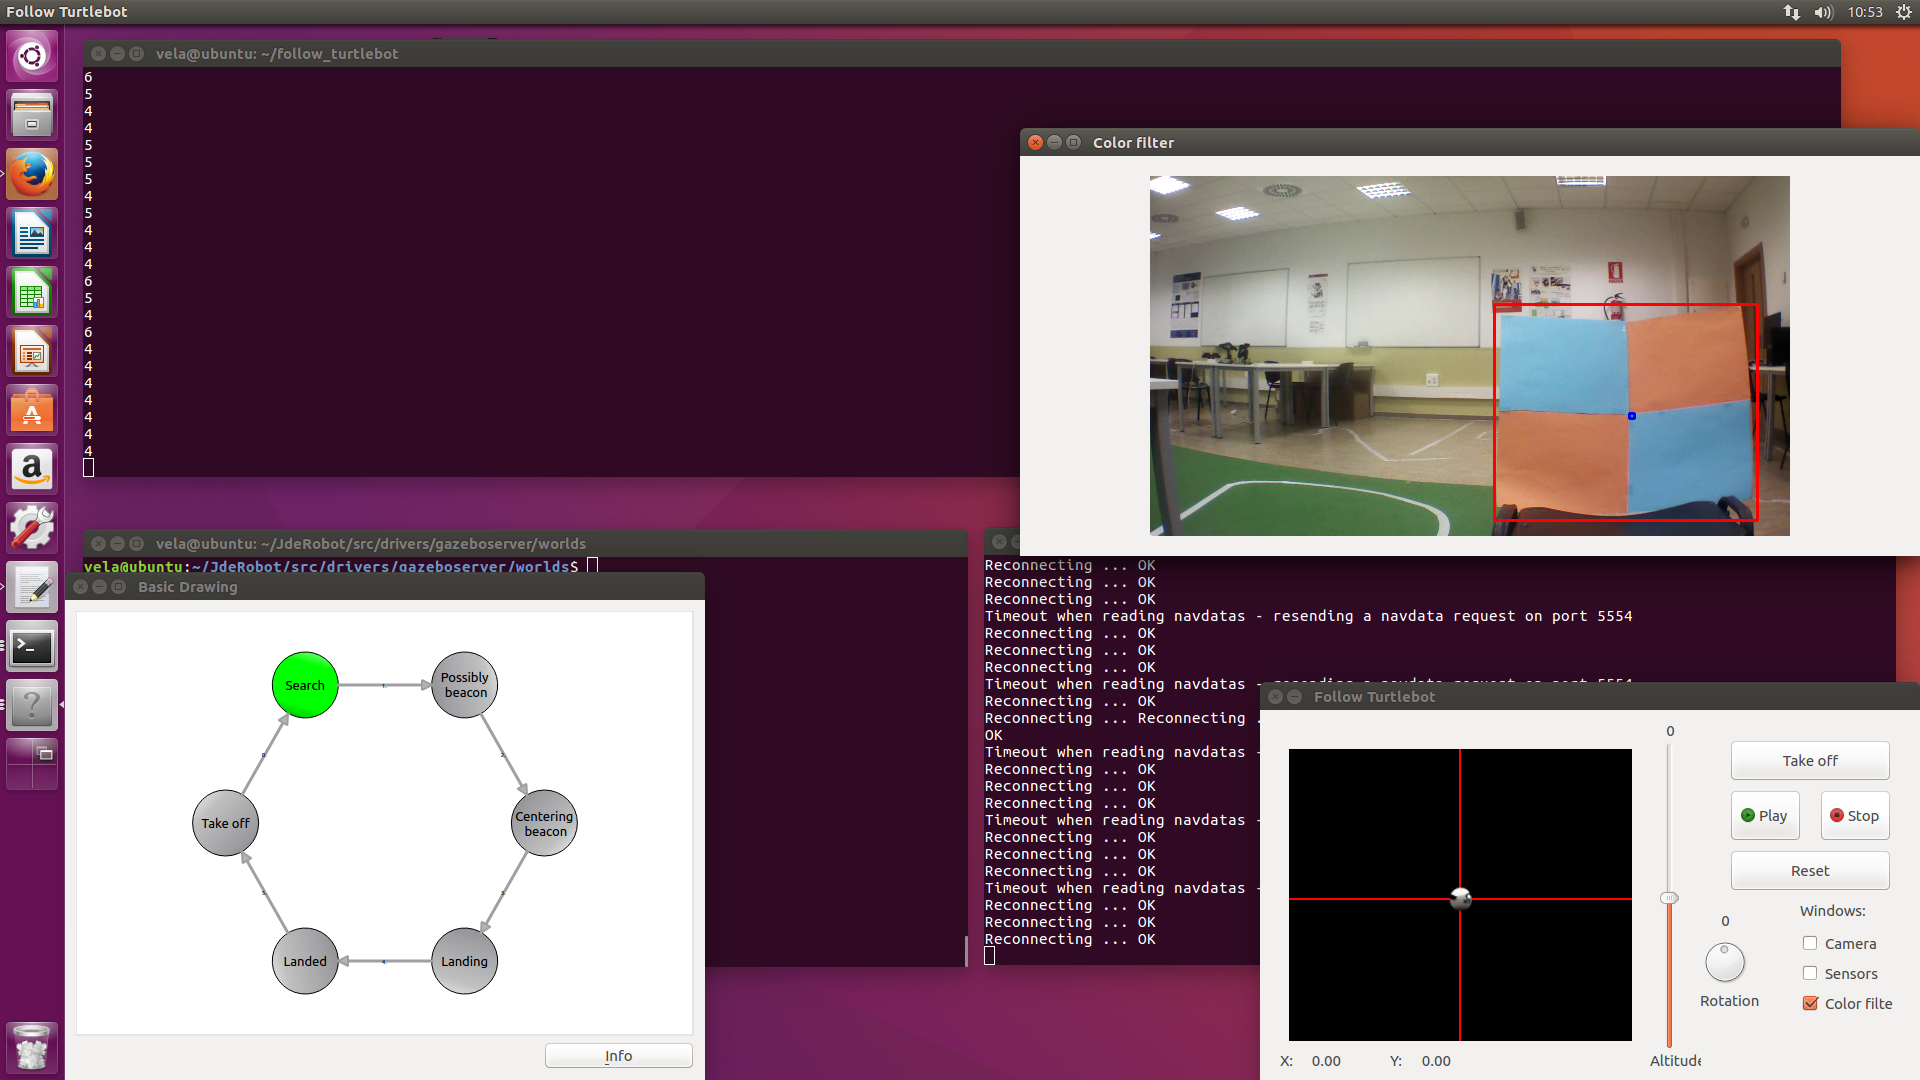
\includegraphics[width=1.0\textwidth]{C:/Users/jorge/Pictures/k_beacon2.eps}
		\caption{Esta imagen muestra el conjunto de herramientas utilizadas.}
	\label{fig:Herramientas}
\end{figure}


\hspace{1 cm} Ya por \'ultimo, decir lo utilizado para programar el algoritmo. Este se ha desarrollado utilizando Python, gracias al cual hemos podido utilizar bibliotecas como PIL o OpenCV principalmente para el manejo de im\'agenes. Nos permit\'ian obtener la imagen transmitida por el dron con facilidad y aplicarle los filtros de color deseados en cada momento, as\'i como realizar realizar distintas operaciones morfol\'ogicas (erosi\'on , dilataci\'on, apertura y cierre) sobre los fotogramas en cada momento, obteniendo im\'agenes m\'as claras sobre las cuales podemos trabajar y con sus funciones, como puede ser drawcontours, obtener un c\'odigo m\'as compacto y eficiente. Esto nos permite un mejor rendimiento del algoritmo, lo que nos llevar\'a a unos mejores resultados. 


\end{document}